\section{Introduction}

% It is a challenging testbed for robotics algorithms
Table tennis is a challenging game for humans to master. For robots, it also serves as a testbed to study and validate the effectiveness of different movement generation algorithms. Combining different estimation, movement generation and execution schemes and studying how close they come to imitating expert human behaviour will yield important insights for robotics research.

Optimality plays an important role in the search for efficient and feasible striking trajectories. However, so far most of the research in robotic table tennis were based on specialized systems, such as Cartesian coordinate robots \citep{Matsushima05,Yanlong13}, that eliminate great part of the difficulties in trajectory generation. Furthermore, most algorithms for robotic table tennis focused on simplifications of the game that reduced the dimensions of the search space \citep{Muelling11} in order to quickly come up with a movement plan. In this paper, we show the advantages of incorporating optimality in trajectory generation to create more flexible movement. 
% refs needed

% GOOD SOUNDS A BIT INFORMAL
Our robotic setup with an anthropomorphic seven degree of freedom Barrett WAM arm is shown in Figure~\ref{robot}. The redundant arm can achieve high speeds and accelerations. It is a good platform to study different movement generation schemes. Optimal control based approaches have the potential to make use of all degrees of freedom in planning, contributing to more natural and efficient generation of strikes. % ref needed
%
The contributions of this paper are as follows: first, we introduce an optimal control framework in robot table tennis where the generation of striking trajectories is the result of an optimization problem. As opposed to previous works, inverse kinematics or a fixed plane to compute joint trajectories are not needed. Two different optimization approaches are presented that encode defensive and goal-oriented styles of playing. We show extensive experiments in simulation and on our table tennis platform, where we evaluate and compare the performance of the algorithms. We do not rely on pure physical modeling to compute desired ball and racket parameters. Instead, the parameters of the prediction models are estimated based on human ball-racket demonstrations.
%
\begin{figure}[t]
	\center
	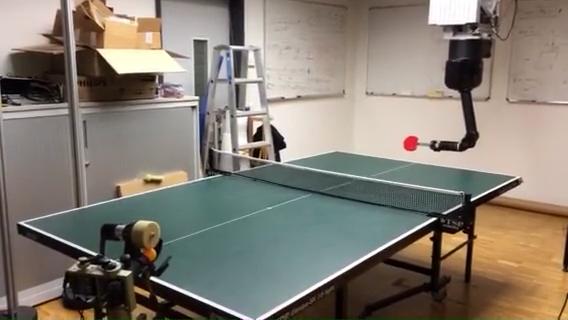
\includegraphics[scale=0.4]{robot1.png}			
	\caption{Robotic table tennis setup with four cameras on the corners of the ceiling tracking the ball at 60 Hz. We present two optimal control based trajectory generation algorithms that encode defensive and goal-oriented styles of playing. A constrained nonlinear optimization problem is solved in both cases to find an optimal striking trajectory as well as an optimal striking time.	
		%The raw ball data provided from the cameras is filtered with an Extended Kalman Filter and the future path of the ball is predicted.
	}
	\label{robot}
\end{figure}